\documentclass[a4paper, 11pt, twoside]{article}

\usepackage{hyperref}
%\usepackage[ngerman]{babel}
\usepackage[english]{babel}
%\usepackage[latin1]{inputenc}
\usepackage[utf8]{inputenc}

\usepackage{graphicx,float,subfigure}
%\usepackage{pifont}
\usepackage{type1cm}
\usepackage{amssymb, amsthm, amsmath}
\usepackage{listings}

\usepackage{pgf}
\usepackage{url}
%\usepackage{graphicx}
%\usepackage{pifont}
%\usepackage{type1cm}
\usepackage{hyperref}

\usepackage{makeidx}
\makeindex

\setlength{\parindent}{0em}
\setlength{\oddsidemargin}{0.0cm}
\setlength{\evensidemargin}{0.0cm}
\setlength{\textheight}{23cm}
\setlength{\topmargin}{-0.5cm}
\setlength{\footskip}{1.5cm}
\setlength{\textwidth}{15.5cm}

\renewcommand*\familydefault{\sfdefault}

\begin{document}
\thispagestyle{empty}

%\documentclass[a4paper]{article}

%\usepackage{pgf}
%\usepackage{graphicx}
%\usepackage{pifont}
%\usepackage{type1cm}

\setlength{\textwidth}{14cm}
\setlength{\oddsidemargin}{1cm}

%\begin{document}

\thispagestyle{empty}

%%%%%%%%%%%%%%%%%%%%%%%%%%%%%%%%%%%%%%%%
%%%%%%%%%%%%%%%%%%%%%%%%%%%%%%%%%%%%%%%%
%%%%%%%%%%%%%%%%%%%%%%%%%%%%%%%%%%%%%%%%

\newcount \Z
\Z=20

%%% logos %%%

%%% NUMHPC %%%
\newlength{\numhpclogox}
\setlength{\numhpclogox}{\paperwidth} % 20/210ths of the paperwidth
\divide\numhpclogox by 210
\multiply\numhpclogox by 100

\newlength{\numhpclogoy}
\setlength{\numhpclogoy}{\paperheight} % 270/297ths of the paperwidth
\divide \numhpclogoy by 297
\multiply \numhpclogoy by -235

\newlength{\numhpclogoheight}
\setlength{\numhpclogoheight}{\paperheight} % 270/297ths of the paperwidth
\divide\numhpclogoheight by 297
\multiply\numhpclogoheight by 20

%%% KIT %%%
\newlength{\kitlogox}
\setlength{\kitlogox}{\paperwidth} % 20/210ths of the paperwidth
\divide\kitlogox by 210
\multiply\kitlogox by 0

\newlength{\kitlogoy}
\setlength{\kitlogoy}{\paperheight} % 270/297ths of the paperwidth
\divide \kitlogoy by 297
\multiply \kitlogoy by -230

\newlength{\kitlogoheight}
\setlength{\kitlogoheight}{\paperheight} % 270/297ths of the paperwidth
\divide\kitlogoheight by 297
\multiply\kitlogoheight by 15


%%% EMCL %%%
\newlength{\emcllogox}
\setlength{\emcllogox}{\paperwidth} % 20/210ths of the paperwidth
\divide\emcllogox by 210
\multiply\emcllogox by 28

\newlength{\emcllogoy}
\setlength{\emcllogoy}{\paperheight} % 270/297ths of the paperwidth
\divide \emcllogoy by 297
\multiply \emcllogoy by -160

\newlength{\emcllogoheight}
\setlength{\emcllogoheight}{\paperheight} % 270/297ths of the paperwidth
\divide\emcllogoheight by 297
\multiply\emcllogoheight by 20

%%% HIFLOW %%%
\newlength{\hiflowlogox}
\setlength{\hiflowlogox}{\paperwidth} % 20/210ths of the paperwidth
\divide\hiflowlogox by 210
\multiply\hiflowlogox by 28

\newlength{\hiflowlogoy}
\setlength{\hiflowlogoy}{\paperheight} % 270/297ths of the paperwidth
\divide \hiflowlogoy by 297
\multiply \hiflowlogoy by -160

\newlength{\hiflowlogoheight}
\setlength{\hiflowlogoheight}{\paperheight} % 270/297ths of the paperwidth
\divide\hiflowlogoheight by 297
\multiply\hiflowlogoheight by 33

%%%%%%%%%%%%%%%%%%%%%%%%%%%%%%%%%%%%%%%%
%%%%%%%%%%%%%%%%%%%%%%%%%%%%%%%%%%%%%%%%
%%%%%%%%%%%%%%%%%%%%%%%%%%%%%%%%%%%%%%%%

%%% NUMHPC %%%
%%\pgftext[bottom, left, at={\pgfpointadd{\pgfpoint{0pt}{0pt}}{\pgfpoint{\numhpclogox}{\numhpclogoy}}}]{\includegraphics[totalheight=\numhpclogoheight]{numhpc}}

%%% KIT %%%
%%\pgftext[bottom, left, at={\pgfpointadd{\pgfpoint{0pt}{0pt}}{\pgfpoint{\kitlogox}{\kitlogoy}}}]{\includegraphics[totalheight=\kitlogoheight]{kitlogo}}

%%% EMCL %%%
\pgftext[bottom, left, at={\pgfpointadd{\pgfpoint{0pt}{0pt}}{\pgfpoint{\hiflowlogox}{\hiflowlogoy}}}]{
\includegraphics[totalheight=\hiflowlogoheight]{HF3_color}}

%%% horizontal lines %%%
\pgfline{\pgfxy(-1pt,0.1pt)}{\pgfxy(15pt,0.1pt)}
\pgfline{\pgfxy(-1pt,-21.4pt)}{\pgfxy(15pt,-21.4pt)}
%%\pgfline{\pgfxy(-1pt,-22.4pt)}{\pgfxy(15pt,-22.4pt)}

%%% EMCL text %%%
\pgftext[bottom, left, at={\pgfpointadd{\pgfpoint{0pt}{0pt}}{\pgfpoint{0cm}{1cm}}}]{{\LARGE{{\bf Tutorial}}}}

%%% EMCL web %%%
\pgftext[bottom, left, at={\pgfpointadd{\pgfpoint{0pt}{0pt}}{\pgfpoint{10.5cm}{-21.7cm}}}]{{\fontsize{13}{10}\selectfont{} http://www.hiflow3.org/}}

\hspace{2cm}
\begin{picture}(0,0)(-250,-25)

\includegraphics[scale=.22]{emcl.pdf} 
\end{picture}

%%% author %%%
\pgftext[bottom, left, at={\pgfpointadd{\pgfpoint{0pt}{0pt}}{\pgfpoint{0cm}{-4cm}}}]{{
\begin{parbox}{13cm}{
\begin{center}\fontsize{12}{30}\selectfont{} Julian Kr\"amer
\end{center}}
\end{parbox}}}

%%% title %%%
\pgftext[bottom, left, at={\pgfpointadd{\pgfpoint{0pt}{0pt}}{\pgfpoint{0cm}{-7.5cm}}}]{{
\begin{parbox}{13cm}{
%%\begin{center}\fontsize{18}{30}\selectfont{} \bf Using HiFlow$^3$ for solving the
\begin{center}\fontsize{22}{30}\selectfont{} \bf Distributed Control Problem\\ for Poisson Equation
\end{center}}
\end{parbox}}}

%%% date %%%
\pgftext[bottom, left, at={\pgfpointadd{\pgfpoint{0pt}{0pt}}{\pgfpoint{0cm}{-16.4cm}}}]{{
\begin{parbox}{13cm}{
\begin{center}\fontsize{12}{24}\selectfont{} 
\vspace{5cm}
\textit{modified on \today}\\ 
\vspace{6.5cm}
\hspace{6cm}\textit{Version 1.3}
\end{center}}
\end{parbox}}}

%fhfh \hfill sjdh

%\end{document}


%\newpage
%\null\newpage

\newcommand{\dd}{\mathrm{d}}
\newtheorem{remark}{Remark}[section]
\thispagestyle{empty}
\tableofcontents

\newpage
\pagestyle{plain}
\framebox[15.5cm]{\parbox[c][2.3cm]{14.0cm}{
{\fontsize{19}{30}\selectfont{} \bf{Applying HiFlow$^3$ for solving the distributed control problem for Poisson equation}
}}}
\vspace{0.5cm}
\section{Introduction}

HiFlow$^3$ is a multi-purpose finite element software providing powerful tools for efficient and accurate solution of a wide range of problems modeled by partial differential equations (PDEs). Based on object-oriented concepts and the full capabilities of C++ the HiFlow$^3$ project follows a modular and generic approach for building efficient parallel numerical solvers. It provides highly capable modules dealing with the mesh setup, finite element spaces, degrees of freedom, linear algebra routines, numerical solvers, and output data for visualization. Parallelism - as the basis for high performance simulations on modern computing systems - is introduced on two levels: coarse-grained parallelism by means of distributed grids and distributed data structures, and fine-grained parallelism by means of platform-optimized linear algebra back-ends.
About this tutorial: Since we discuss an optimization problem with the Poisson equation as a constraint, this tutorial is closely related to the Poisson tutorial which you can find on the Hiflow$^3$ webpage. Therefore a few details in the theoretical part are omitted here, but you will find references to the corresponding section of the Poisson tutorial.

\subsection{How to Use the Tutorial?}
You find the example code (distributed\_control\_poisson\_tutorial.cc, \\ 
distributed\_control\_poisson\_tutorial.h), a parameter file for the first numerical example\\ (distributed\_control\_poisson\_tutorial.xml)  
and a Makefile, which you only need when using HiFlow$^3$ as a library (see \ref{sectionlibrary}), in the folder \verb'/hiflow/examples/distributed_control_poisson'. The geometry data (*.inp, *.vtu) is stored in the folder \verb'/hiflow/examples/data'.

\subsubsection{Using HiFlow$^3$ as a Library}\label{sectionlibrary}
First install HiFlow$^3$. Therefore, follow the instructions listed on \verb'http://www.hiflow3.org/', see "Documentation"-"Installation".
To compile and link the tutorial correctly, you may have to adapt the Makefile depending on the options you chose in the cmake set up. Make sure that the variable \verb'HIFLOW_DIR' is set to the path, where HiFlow$^3$ was installed. The default value is \verb'/usr/local'. Additionally, when you have installed HiFlow$^3$ with ILU++, make sure that the variable \verb'ILU_DIR' is set to the path where ILU++ was installed (\href{http://iamlasun8.mathematik.uni-karlsruhe.de/~ae04/iluplusplus_introduction.html}{ILU++}). You install HiFlow$^3$ with ILU++ by setting the option \verb'WANT_ILUPP' to \verb'ON' in the cmake set up. When you want to install it with metis, you have to set the option \verb'WANT_METIS' to \verb'ON' (\href{http://www.cs.umn.edu/~metis}{metis}). If you have installed one of these or both, you have to follow the instructions in the Makefile and uncomment the necessary lines to link metis or ILU++. By typing \verb'make' in the console, in the same folder where the source-code and the Makefile is stored, you compile and link the tutorial. 
To execute the distributed control Poisson tutorial sequentially, type \textbf{./distributed\_control\_poisson\_tutorial} \verb'/"path_to"/distributed_control_poisson_'\\ \verb'tutorial.xml' \verb'/"path_to_mesh_data"/' . To execute it in parallel mode \index{program!executing in parallel} with four processes type \textbf{mpirun -np 4 ./distributed\_control\_poisson\_tutorial} \verb'/"path_to"/distributed_'\\ \verb'control_poisson_tutorial.xml' \verb'/"path_to_mesh_data"/' . 
 This tutorial is currently implemented in 1D, 2D and 3D. Note that for 1D only the sequential mode is available. To change the dimension simply change the integer 'Dimension' in line 35 of distributed\_control\_poisson\_tutorial.h. A suitable mesh and right-hand side are automatically chosen.

\subsubsection{Using HiFlow$^3$ as a Developer}\label{sectiondeveloper}
First build and compile HiFlow$^3$. Go to the directory \verb'/build/example/distributed_control'\\ \verb'_poisson', where the binary \textbf{distributed\_control\_poisson\_tutorial} is stored. Type \\ \textbf{./distributed\_control\_poisson\_tutorial}, to execute the program in sequential mode. To execute in parallel mode \index{program!executing in parallel} with four processes, type \textbf{mpirun -np 4 ./distributed\_control\_poisson\_tutorial}. In both cases, you need to make sure that the default parameterfile distributed\_control\_poisson\ \\ \_tutorial.xml is stored in the same directory as the binary, and that the geometry data specified in the parameter file is stored in \verb'/hiflow/examples/data'. Alternatively, you can specify the path of your own xml-file with the name of your xml-file (first) and the path of your geometry data (second) in the comment line, i.e. \textbf{./distributed\_control\_poisson\_tutorial} \verb'/"path_to_parameterfile"/'\\ \verb'"name_of_parameterfile".xml' \verb'/"path_to_geometry_data"/'.


\section{Mathematical Setup}
For simplification, we explain the mathematical setup only for the two dimensional case. However, it is easy to expand the theory to one or three dimensions. \\
\subsection{Problem}
Our aim is to find the state $y \in C^2(\Omega)$ and the control $u \in C^0(\Omega)$ that minimize the cost functional
\begin{equation}\label{objectivefunctional}
 \underset{y, u}{\text{min}} ~J(y,u)=\frac{1}{2} \|y-y_{\Omega}\|^2_{L^2(\Omega)}+\frac{\lambda}{2}\|u\|^2_{L^2(\Omega)}
\end{equation} 
subject to
\begin{eqnarray}\label{conditions}
\begin{array}{rcll}
-\Delta y &=& f+u, & \text{ in }\Omega,\\
        y&=& 0, & \text{ on }\partial\Omega, \\

\end{array}
\end{eqnarray}
where $\Omega \in \mathbb{R} ^2$ is a bounded Lipschitz-domain, $\lambda > 0$  is a real number, $f \in C^0(\Omega)$, $y_{\Omega}$ is the desired state of $y$ and $u$ its control. $\lambda$ is needed for regularization of $u$. \\
The emerging problem is stationary, i.e. it does not depend on time. It can be interpreted as the result of a heating process after some time passed, where all time derivatives of y are zero, that means an equilibrium is reached and the state does not change anymore. Because $u$ is defined on $\Omega$ this correlates for example to the heating process in a microwave. If $u$ would only act on the boundary of $\Omega$ it would correlate for instance to the process in an oven. \\


\subsection{Weak Formulation}\label{sectionWeak_formulation}

In the Hilbert space $L^2(\Omega)$ we can reformulate equation (\ref{conditions}) in a weaker sense: \\
Find $y \in C^2(\Omega)$, $u \in C^0(\Omega)$ such that for all test functions $\varphi\in L^\infty_0(\Omega)$ it holds:

\begin{eqnarray}\label{var_formulation}
\begin{array}{rcl}
\int_\Omega - \Delta y\, \varphi\, \dd x &=& \int_\Omega f\varphi\, \dd x + \int_\Omega u\varphi\, \dd x. \\
\end{array}
\end{eqnarray}




Using Green's first identity and the Gaussian integral theorem, we get
\begin{eqnarray}\label{var_formulationgreen}
\begin{array}{rcl}
\int_\Omega \nabla y\cdot \nabla\varphi\, \dd x - \int_{\partial\Omega} (\nabla y \cdot n) \varphi \dd \sigma &=& \int_\Omega f\varphi\, \dd x + \int_\Omega u\varphi\, \dd x , \\

\end{array}
\end{eqnarray}
where $n$ is the (outer) normal vector on $\partial \Omega$. Since the test functions $\varphi$ have compact support in $\Omega$, and therefore $\varphi=0$ on $\partial \Omega$, we get from (\ref{var_formulationgreen}) that
\begin{eqnarray}\label{var_formulation2}
\begin{array}{rcll}
\int_\Omega \nabla y\cdot \nabla\varphi\, \dd x  &=& \int_\Omega f\varphi\, \dd x + \int_\Omega u\varphi\, \dd x & \forall \varphi\in H_0^1(\Omega). \\
\end{array}
\end{eqnarray}
Now $y$ and $\varphi$ can be chosen from $H^1_0(\Omega)$ since no second derivative is required anymore and $u$ can be chosen from $L^2(\Omega)$ since no derivative is necessary. Such an $(y, u) \in H^1_0(\Omega)\times L^2(\Omega)$ minimizing \ref{objectivefunctional} subject to \ref{var_formulation2} is called a $\mathit{weak}$ solution \index{solution!weak} of the problem (\ref{objectivefunctional}) + (\ref{conditions}). \\
The bilinear form 
\[
a: H^1_0(\Omega) \times H^1_0(\Omega) \rightarrow \mathbb{R},\quad a(y,\varphi)=\int_\Omega \nabla y \cdot \nabla\varphi\, \dd x  
\]
is continuous and elliptic. Therefore, by Lax-Milgram lemma,\index{Lax-Milgram theorem} the equation (\ref{var_formulation2})
has one and only one state $y$ for a given $u$, see \cite[Chap 5.8]{gilbarg} or \cite{mclean}\index{solution!uniqueness} \index{solution!existence}. The Cea lemma,\index{Cea lemma} see \cite[Chap. 2.8, 2.5]{brenner}, represents the analogon of the Lax-Milgram theorem for finite dimensional spaces. 
That means, the coercivity of the bilinear form $a$ transfers from $H^1_0(\Omega)$ onto finite dimensional subspace $H_h(\Omega) \subseteq H^1_0(\Omega)$. \\
Now that we weakened the assumptions on our problem, the next question is what conditions need to be satisfied that a given solution is optimal. \\

\subsection{Existence of optimal solutions}

Since there is for every possible $u$ exactly one weak solution $y$, we reformulate $y:= y(u)$, to express its dependency on u. In other words: $u$ determines the shape of y in a unique way. \\
A control $u^*$ is called optimal if the cost functional
\begin{eqnarray}\label{optimality_condition}
\begin{array}{rll}
J(y(u^*), u^*) \le J(y(u), u) & \text{for all possible} & u
\end{array}
\end{eqnarray}
and one can show that there is an operator 
\[
S: u \mapsto y(u), S:L^2(\Omega) \rightarrow L^2(\Omega),
\]
which is linear and continuous (\cite[Chap. 2.5.1]{troeltzsch}). With this operator, we reduce the cost functional $J(y , u)$ to $J(u)$ and get
\begin{eqnarray}\label{costfunctional_u}
 \underset{u}{\text{min}} ~J(u)=\frac{1}{2} \|Su-y_{\Omega}\|^2_{L^2(\Omega)}+\frac{\lambda}{2}\|u\|^2_{L^2(\Omega)}
\end{eqnarray}
This optimality problem has at least one optimal solution $u^*$, if the set $U$ of all possible $u$ is convex, not empty and bounded, which is the case for $U = L^2(\Omega)$. Furthermore it has exactly one optimal solution $u^*$ if also $\lambda > 0$. \\
With this optimal solution, we can deduce the Karush-Kuhn-Tucker system. In the next section this is done with the Langrange ansatz.
(\cite[Chap. 2.10]{troeltzsch})



\subsection{Optimality System}\label{sectionoptimalsystem}\index{lagrange}
We define the Lagrange equation for the problem (\ref{objectivefunctional}) + (\ref{var_formulation2}) by 

\begin{eqnarray}\label{Lagrange equation}
L(y,u,p) = J(y,u) - (\int_\Omega \nabla y\cdot \nabla p \, \dd x  - \int_\Omega f p \, \dd x - \int_\Omega u p\, \dd x) \cdot 
\end{eqnarray}
where $p \in H^1(\Omega)$ is the Lagrangian multiplier. The necessary condition for an optimal solution, if we have no constraints for $u$, is that the partial derivations of the Langrange functional are zero, i.e.

\begin{eqnarray}\label{Lagrangederivatives}
\begin{array}{c}
\partial_y L(y,u,p) = 0, \\
\partial_u L(y,u,p) = 0, \\
\partial_p L(y,u,p) = 0.
\end{array}
\end{eqnarray}
In this case, equations (\ref{Lagrangederivatives}) lead to the optimality system: Find $y, p \in H^1_0(\Omega), u \in L^2(\Omega)$ such that

\begin{eqnarray}\label{optimalsystem}\index{optimal system}
\begin{array}{rcll}
\int_\Omega \nabla y\cdot \nabla\varphi\, \dd x &=& \int_\Omega f\varphi\, \dd x + \int_\Omega u\varphi\, \dd x & \forall \varphi\in H_0^1(\Omega), \\
\int_\Omega \nabla p\cdot \nabla\psi\, \dd x &=& \int_\Omega y\psi\, \dd x -\int_\Omega y_{\Omega}\psi\, \dd x & \forall \psi\in H_0^1(\Omega), \\		
\lambda \int_\Omega u\mu\, \dd x + \int_\Omega p\mu\, \dd x &=& 0 & \forall \mu\in L^2(\Omega). \\
\end{array}
\end{eqnarray}
Since the problem is convex, the necessary conditions are also sufficient. Hence, we need to solve the optimality system. The triple $\{y^*, p^*, u^*\}$ that solves system (\ref{optimalsystem}) is optimal and $u^*$ is called the optimal control.


\subsection{Resulting Matrix}
The next step is the discretization of the problem. We choose a set of finite dimensional basis functions and approximate y, u and p with a sum over those basis functions \cite[Chap. 2.12]{troeltzsch}:

\begin{eqnarray}
\begin{array}{rcl}

y(x) &=& \sum_{i=1}^N y_i \varphi_i , \\
p(x) &=& \sum_{i=1}^N p_i \psi_i  , \\
u(x) &=& \sum_{i=1}^N u_i \mu_i ,
\end{array}
\end{eqnarray}
where $N \in \mathbb{R}$ is the number of degrees of freedom of each variable. Since we use piecewise linear (resp. bilinear) ansatz functions to discretize $H_h(\Omega) \subseteq H^1_0(\Omega)$ and $L_h(\Omega) \subseteq L^2(\Omega)$, each variable is discretized by the number of degrees of freedom $N$ . We now choose the same basis functions for the test functions and get for example for the first equation of (\ref{optimalsystem})

\begin{eqnarray}
\mathcal{A} y - \mathcal{M} u = 0
\end{eqnarray}

where $\mathcal A$ has the entries $a_{ij} = \int_\Omega \nabla \varphi_i \nabla \varphi_j \dd x$ and $\mathcal M$ has the entries $m_{ij} = \int_\Omega \varphi_i \varphi_j \dd x$. $\mathcal A$ is called the stiffness matrix and $\mathcal M$ is called the mass matrix. For the whole system (\ref{optimalsystem}) we get 
\begin{eqnarray}\label{linearsystem}\index{linear system}
\begin{pmatrix}
\mathcal A & 0 & -\mathcal M \\
-\mathcal M &\mathcal A & 0 \\
0 & -\mathcal M & -\lambda \mathcal M 
\end{pmatrix}
\begin{pmatrix}
y \\
p \\
u
\end{pmatrix}
=
\begin{pmatrix}
\mathcal M f \\
- \mathcal My_\Omega \\
0
\end{pmatrix}
\end{eqnarray}



To simplify the resulting system of linear equations, we choose hat functions of the form

\begin{equation}\index{hat functions}
\phi_i =
\left\{
	\begin{array}{ll}
		1  & \mbox{if } i = j \\
		0 & \mbox{else } 
	\end{array}
	\text{for } j = 1,2,..N
\right.
\end{equation}
as a base, where $N$ is the number of the degrees of freedom. Now only a few entries of the stiffness matrices and mass matrices are nonzero. (\ref{linearsystem}) is then solved by one of the implemented linear solvers in Hiflow$^3$. Since the system matrix is not positive definite, the GMRES method is a good choice.



\subsection{Suitability of the weak formulation}
See Poisson tutorial, Chap. 2.4 for more detail about the relation between strong and weak formulation of the problem. The results from that chapter can be transfered to our optimal control problem. Therefore the weak solution can be viewed assuming additional regularity as a classical one.



\section{The Commented Program}
\subsection{Preliminaries}
HiFlow$^3$ is designed for high performance computing on massively parallel machines. 
So it applies the Message Passing Interface (MPI)\index{Message Passing Interface (MPI)}\index{MPI} library specification for message-passing, see sections \ref{sectionmain}, \ref{read-mesh}, \ref{memberComputeError}, \ref{adapt}, \cite{MPI}, \cite{MPIstandard} .\\
The distributed control Poisson tutorial needs following two input files:
\begin{itemize}
\item A parameter file: The parameter file is an xml-file, which contains all parameters needed to execute the program. It is read in by the program. It is not necessary to recompile the program, when parameters in the xml-file are changed. By default the distributed control Poisson tutorial reads in the parameter file distributed\_control\_poisson\_tutorial.xml, see section \ref{sectionparameter file}, which contains the parameters of the numerical example, see section \ref{sectionExample}. This file is stored in \verb'/hiflow/examples/distributed_control_poisson/'.  
\item Geometry data\index{geometry data}: The file containing the geometry is specified in the parameter file (distributed\_control\_poisson\_tutorial.xml). In the numerical example in section \ref{sectionExample} we used \textbf{unit\_line.inp}, \textbf{unit\_square.inp} and \textbf{unit\_cube.inp}. You can find different meshes in the folder \verb'/hiflow/examples/data' .
\end{itemize}

HiFlow$^3$ does not generate meshes\index{mesh!generate} for the domain $\Omega$.\index{domain geometry!generating} Meshes in *.inp and *.vtu format can be read in. 
It is possible to extend the reader for other formats.
Furthermore it is possible to generate other geometries by using external programs (Mesh generators) or by hand.\\  

\subsection{Parameter File}\index{parameter file}\label{sectionparameter file}
The needed parameters are initialized in the parameter file distributed\_control\_poisson\_tutorial.xml.
\begin{lstlisting}[language=C++, basicstyle={\footnotesize, \ttfamily}, keywordstyle=\color{blue}, numbers=none, tabsize=4]
<Param>	
  <General>
    <Lambda>0.0001</Lambda>
  </General>
  <Mesh>
    <Filename1>unit_line.inp</Filename1>
    <Filename2>unit_square.inp</Filename2>
    <Filename3>unit_cube.inp</Filename3>
    <InitialRefLevel>3</InitialRefLevel>
    <FinalRefLevel>8</FinalRefLevel>
    <FeDegreey>1</FeDegreey>
    <FeDegreep>1</FeDegreep>
    <FeDegreeu>1</FeDegreeu>
  </Mesh>
  <LinearAlgebra>
    <NameMatrix>CoupledMatrix</NameMatrix>
    <NameVector>CoupledVector</NameVector>
    <Platform>CPU</Platform>
    <Implementation>Naive</Implementation>
    <MatrixFormat>CSR</MatrixFormat>
  </LinearAlgebra>
  <LinearSolver>
    <Name>GMRES</Name>
    <SizeBasis>50</SizeBasis>
    <Method>NoPreconditioning</Method>
    <MaxIterations>10000</MaxIterations>
    <AbsTolerance>1.0e-14</AbsTolerance>
    <RelTolerance>1.0e-8</RelTolerance>
    <DivTolerance>1.0e6</DivTolerance>
  </LinearSolver>
    <ILUPP>
    <PreprocessingType>0</PreprocessingType>
    <PreconditionerNumber>1000</PreconditionerNumber>
    <MaxMultilevels>20</MaxMultilevels>
    <MemFactor>0.8</MemFactor>
    <PivotThreshold>17.5</PivotThreshold>
    <MinPivot>0.01</MinPivot>
  </ILUPP>
</Param>
\end{lstlisting}

\subsection{Structure of the Distributed Control Poisson Tutorial}
Following member functions (signed by \textbullet) are defined in the class DistributedControlPoissonTutorial. The survey reflects the  access relations between the functions, classes and structs. 
 \begin{itemize}
    \item run()
    \item build\_initial\_mesh()
    \item prepare\_system()
    \begin{itemize}
	\item DirichletZero-struct (distributed\_control\_poisson\_tutorial.h)
    \end{itemize}
    \item assemble\_system()
    \begin{itemize}
	\item LocalDistributedControlPoissonAssembler-class (distributed\_control\_poisson\_tutorial.h)
        \begin{itemize}
	    \item ExactSol-struct (distributed\_control\_poisson\_tutorial.h)
	\end{itemize}    
    \end{itemize}    
    \item solve\_system()
    \item compute\_error()
    \begin{itemize}
	\item L2ErrorIntegrator-class (distributed\_control\_poisson\_tutorial.h)
	\item H1ErrorIntegrator-class (distributed\_control\_poisson\_tutorial.h)    
    \end{itemize}  
    \item visualise()
    \item adapt()
 \end{itemize} 
You can find the source code of every member function  in an extra section below. 

%\subsection{Source text variables}
%...

\subsection{Main Function}\index{MPI}\label{sectionmain}
The main function starts the simulation of the distributed control Poisson problem \\
(distributed\_control\_poisson\_tutorial.cc).

\begin{lstlisting}[language=C++, basicstyle={\footnotesize, \ttfamily}, keywordstyle=\color{blue}, numbers=none, tabsize=4]
int main ( int argc, char** argv )
{
    MPI_Init ( &argc, &argv );

    // set default parameter file
    std::string param_filename ( PARAM_FILENAME );
    std::string path_mesh;
    // if set take parameter file specified on console
    if ( argc > 1 )
    {
        param_filename = std::string ( argv[1] );
    }
    // if set take mesh following path specified on console
    if ( argc > 2 )
    {
        path_mesh = std::string ( argv[2] );
    }
    try
    {
        // Create log files for INFO and DEBUG output
        std::ofstream info_log ( 
               "distributed_control_poisson_tutorial_info_log" );
        LogKeeper::get_log ( "info" ).set_target ( &info_log );
        std::ofstream debug_log ( 
               "distributed_control_poisson_tutorial_debug_log" );
        LogKeeper::get_log ( "debug" ).set_target ( &debug_log );

        // Create application object and run it
        DistributedControlPoisson app ( param_filename, path_mesh );
        app.run ( );
    }
    catch ( std::exception& e )
    {
        std::cerr << "\nProgram ended with uncaught exception.\n";
        std::cerr << e.what ( ) << "\n";
        return -1;
    }
    MPI_Finalize ( );
    return 0;
}
\end{lstlisting}

\subsection{Member Functions}
\subsubsection{run()}
The member function run() is defined in the class DistributedControlPoissonTutorial \\
(distributed\_control\_poisson\_tutorial.cc).

\begin{lstlisting}[language=C++, basicstyle={\footnotesize, \ttfamily}, keywordstyle=\color{blue}, numbers=none, tabsize=4]
    void run ( )
    {
        // Construct / read in the initial mesh.
        build_initial_mesh ( );

        // Main adaptation loop.
        while ( !is_done_ )
        {
            // Initialize space and linear algebra.
            prepare_system ( );
            // Compute the stiffness matrix and right-hand side.
            assemble_system ( );
            // Solve the linear system.
            solve_system ( );
            // Compute the error to the exact solution.
            compute_error ( );
            // Visualize the solution and the errors.
            visualize ( );
            // Modify the space through refinement. 
            // Set is_done_ = true when finished.
            adapt ( );
        }
    }
\end{lstlisting}


\subsubsection{build\_initial\_mesh()}\index{MPI}\label{read-mesh}
This member function, defined in the class DistributedControlPoissonTutorial, reads the initial mesh (distributed\_control\_poisson\_tutorial.cc), partitions and distributes the mesh if indicated, and writes out the refined mesh of the initial refinement level.

\begin{lstlisting}[language=C++, basicstyle={\footnotesize, \ttfamily}, keywordstyle=\color{blue}, numbers=none, tabsize=4]
void DistributedControlPoisson::build_initial_mesh ( )
{
    // Read in the mesh on the master process. The mesh is chosen according to
    // the dimension of the problem.
    if ( rank_ == MASTER_RANK )
    {
        std::string mesh_name;
        switch ( DIMENSION )
        {
            case 1:
            {
                mesh_name =
                        params_["Mesh"]["Filename1"].get<std::string>( );
                break;
            }
            case 2:
            {
                mesh_name =
                        params_["Mesh"]["Filename2"].get<std::string>( );
                break;
            }
            case 3:
            {
                mesh_name =
                        params_["Mesh"]["Filename3"].get<std::string>( );
                break;
            }
            default: assert ( 0 );
        }
        std::string mesh_filename;
        if ( path_mesh.empty ( ) )
        {
            mesh_filename = std::string ( DATADIR ) + mesh_name;
        }
        else
        {
            mesh_filename = path_mesh + mesh_name;
        }
        master_mesh_ = read_mesh_from_file ( mesh_filename, DIMENSION,
                                             DIMENSION, 0 );

        // Refine the mesh until the initial refinement level is reached.
        const int initial_ref_lvl = params_["Mesh"]["InitialRefLevel"].
                get<int>( );
        for ( int r = 0; r < initial_ref_lvl; ++r )
        {
            master_mesh_ = master_mesh_->refine ( );
            ++refinement_level_;
        }
    }

    // 1D parallel execution is not yet implemented.
    if ( DIMENSION == 1 )
    {
        mesh_ = master_mesh_;
    }
    else
    {
        MPI_Bcast ( &refinement_level_, 1, MPI_INT, MASTER_RANK, comm_ );

        // Distribute mesh over all processes, and compute ghost cells
        MeshPtr local_mesh = partition_and_distribute ( master_mesh_, 
                                                        MASTER_RANK,
                                                        comm_ );
        assert ( local_mesh != 0 );
        SharedVertexTable shared_verts;
        mesh_ = compute_ghost_cells ( *local_mesh, comm_, shared_verts );

        // Write out mesh of initial refinement level
        PVtkWriter writer ( comm_ );
        std::string output_file =
           std::string ( "distributed_control_poisson_tutorial_mesh.pvtu" );
        writer.add_all_attributes ( *mesh_, true );
        writer.write ( output_file.c_str ( ), *mesh_ );
    }
}
\end{lstlisting}

\subsubsection{prepare\_system()}
The member function prepare\_system() initializes the space and the linear algebra \\(distributed\_control\_poisson\_tutorial.cc). The polynomial degree of the finite element functions is set to the parameter "FeDegree" defined in the parameter file. The size and the non-zero pattern of the stiffness matrix matrix\_ is initialized. The vectors for the right-hand side rhs\_, and the solution are initialized and set to a 0-vector of the correct size.

\begin{lstlisting}[language=C++, basicstyle={\footnotesize, \ttfamily}, keywordstyle=\color{blue}, numbers=none, tabsize=4]
void DistributedControlPoisson::prepare_system ( )
{
    // Assign degrees to each element for each variable.
    const int fe_degree_p = params_["Mesh"]["FeDegreep"].get<int>( );
    const int fe_degree_y = params_["Mesh"]["FeDegreey"].get<int>( );
    const int fe_degree_u = params_["Mesh"]["FeDegreeu"].get<int>( );
    std::vector< int > degrees ( 3, 0 );
    degrees[0] = fe_degree_p;
    degrees[1] = fe_degree_y;
    degrees[2] = fe_degree_u;

    // Initialize the VectorSpace object.
    space_.Init ( degrees, *mesh_ );

    // Setup couplings object.
    couplings_.Init ( comm_, space_.dof ( ) );

    // Compute the matrix graph.
    SparsityStructure sparsity;
    global_asm_.compute_sparsity_structure ( space_, sparsity );

    couplings_.InitializeCouplings ( sparsity.off_diagonal_rows,
                                     sparsity.off_diagonal_cols );

    // Setup linear algebra objects.
    CoupledMatrixFactory<Scalar> CoupMaFact;
    matrix_ = CoupMaFact.Get (
            params_["LinearAlgebra"]["NameMatrix"].get<std::string>( ) )->
            params ( params_["LinearAlgebra"] );
    matrix_->Init ( comm_, couplings_ );
    CoupledVectorFactory<Scalar> CoupVecFact;
    rhs_ = CoupVecFact.Get (
            params_["LinearAlgebra"]["NameVector"].get<std::string>( ) )->
            params ( params_["LinearAlgebra"] );
    sol_ = CoupVecFact.Get (
            params_["LinearAlgebra"]["NameVector"].get<std::string>( ) )->
            params ( params_["LinearAlgebra"] );
    rhs_->Init ( comm_, couplings_ );
    sol_->Init ( comm_, couplings_ );

    // Initialize structure of LA objects.
    matrix_->InitStructure ( vec2ptr ( sparsity.diagonal_rows ),
                             vec2ptr ( sparsity.diagonal_cols ),
                             sparsity.diagonal_rows.size ( ),
                             vec2ptr ( sparsity.off_diagonal_rows ),
                             vec2ptr ( sparsity.off_diagonal_cols ),
                             sparsity.off_diagonal_rows.size ( ) );

    rhs_->InitStructure ( );
    sol_->InitStructure ( );

    // Zero all linear algebra objects.
    matrix_->Zeros ( );
    rhs_->Zeros ( );
    sol_->Zeros ( );

    // Compute Dirichlet BC dofs and values using known exact solution.
    dirichlet_dofs_y_.clear ( );
    dirichlet_dofs_p_.clear ( );
    dirichlet_values_.clear ( );

    DirichletZero zero;
    // The function compute_dirichlet_dofs_and_values des not yet work for 1D.
    if ( DIMENSION == 1 )
    {
        dirichlet_values_.resize ( 2, 0.0 );
        dirichlet_dofs_y_.resize ( 0 );
        dirichlet_dofs_p_.resize ( 0 );

        // Loop over all cells.
        for ( EntityIterator facet_it = mesh_->begin ( DIMENSION - 1 ), 
              facet_end =  mesh_->end ( DIMENSION - 1 ); facet_it != facet_end; 
              ++facet_it )
        {

            // Returns the number of neighbors for each cell, to check if it is
            // on the facet.
            const EntityCount num_cell_neighbors =
                    facet_it->num_incident_entities ( DIMENSION );

            if ( num_cell_neighbors == 1 )
            {
                // If it lies on the facet, the corresponding DOF is a
                // Dirichlet DOF and is added to dirichlet_dofs_y_ 
                // or dirichlet_dofs_p, respectively.
                std::vector<int> dof_number_p;
                std::vector<int> dof_number_y;
                space_.dof ( ).get_dofs_on_subentity ( 0, facet_it->begin_incident
                                                       ( DIMENSION )->index ( ), 
                                                       0, facet_it->index ( ), 
                                                       dof_number_p );
                space_.dof ( ).get_dofs_on_subentity ( 1, facet_it->begin_incident
                                                       ( DIMENSION )->index ( ), 
                                                       0, facet_it->index ( ), 
                                                       dof_number_y );
                dirichlet_dofs_y_.push_back ( dof_number_p[0] );
                dirichlet_dofs_p_.push_back ( dof_number_y[0] );
            }
        }
    }
    else
    {
        compute_dirichlet_dofs_and_values ( zero, space_, 0, dirichlet_dofs_p_,
                                            dirichlet_values_ );
        compute_dirichlet_dofs_and_values ( zero, space_, 1, dirichlet_dofs_y_,
                                            dirichlet_values_ );
    }
}
\end{lstlisting}

\textbf{struct DirichletZero} \label{structDirichletZero}\index{boundary condition!modelling}\\
This struct in distributed\_control\_poisson\_tutorial.h defines the homogeneous Dirichlet boundary condition, given in (\ref{conditions}).
\begin{lstlisting}[language=C++, basicstyle={\footnotesize, \ttfamily}, keywordstyle=\color{blue}, numbers=none, tabsize=4]
struct DirichletZero
{

    std::vector<double> evaluate ( const mesh::Entity& face,
                                   const std::vector<Coord>& coords_on_face ) const
    {
        // return array with Dirichlet values for dof:s on boundary face
        return std::vector<double>( coords_on_face.size ( ), 0.0 );
    }
};
\end{lstlisting}

\subsubsection{assemble\_system()}
The member function assemble\_system() computes the system matrix\index{stiffness matrix!assembling} and right-hand side\index{right-hand side!assembling} (distributed\_control\_poisson\_tutorial.cc). The system matrix, right-hand side vector and solution vector are modified to set correct Dirichlet values for the boundary DoFs.

\begin{lstlisting}[language=C++, basicstyle={\footnotesize, \ttfamily}, keywordstyle=\color{blue}, numbers=none, tabsize=4]
void DistributedControlPoisson::assemble_system ( )
{
    // Assemble matrix and right-hand-side vector.
    const double lambda = params_["General"]["Lambda"].get<double>( );
    LocalDistributedControlPoissonAssembler local_asm ( lambda );
    global_asm_.assemble_matrix ( space_, local_asm, *matrix_ );
    global_asm_.assemble_vector ( space_, local_asm, *rhs_ );

    if ( !dirichlet_dofs_p_.empty ( ) )
    {
        // Correct Dirichlet dofs.
        matrix_->diagonalize_rows ( vec2ptr ( dirichlet_dofs_p_ ), 
                                    dirichlet_dofs_p_.size ( ), 1.0 );
        rhs_->SetValues ( vec2ptr ( dirichlet_dofs_p_ ), dirichlet_dofs_p_.size ( ),
                          vec2ptr ( dirichlet_values_ ) );
        sol_->SetValues ( vec2ptr ( dirichlet_dofs_p_ ), dirichlet_dofs_p_.size ( ),
                          vec2ptr ( dirichlet_values_ ) );
    }

    if ( !dirichlet_dofs_y_.empty ( ) )
    {
        // Correct Dirichlet dofs.
        matrix_->diagonalize_rows ( vec2ptr ( dirichlet_dofs_y_ ), 
                                    dirichlet_dofs_y_.size ( ), 1.0 );
        rhs_->SetValues ( vec2ptr ( dirichlet_dofs_y_ ), dirichlet_dofs_y_.size ( ),
                          vec2ptr ( dirichlet_values_ ) );
        sol_->SetValues ( vec2ptr ( dirichlet_dofs_y_ ), dirichlet_dofs_y_.size ( ),
                          vec2ptr ( dirichlet_values_ ) );
    }

    // Communicate modified values outside if-block
    rhs_->UpdateCouplings ( );
    sol_->UpdateCouplings ( );
}
\end{lstlisting} 

\textbf{LocalDistributedControlPoissonAssembler class}\\
This class in distributed\_control\_poisson\_tutorial.h implements the system matrix and right-hand side locally for each cell.

\begin{lstlisting}[language=C++, basicstyle={\footnotesize, \ttfamily}, keywordstyle=\color{blue}, numbers=none, tabsize=4]
class LocalDistributedControlPoissonAssembler : 
                 private AssemblyAssistant<DIMENSION, double>
{
  public:

    LocalDistributedControlPoissonAssembler ( double lambda ) : lambda_ ( lambda )
    {
    }

    void operator() ( const Element<double>& element, 
                      const Quadrature<double>& quadrature,
                      LocalMatrix& lm )
    {
        AssemblyAssistant<DIMENSION, double>::initialize_for_element ( element, 
                                                                    quadrature );

        // compute local matrix
        lm.Resize ( num_dofs_total ( ), num_dofs_total ( ) );
        lm.Zeros ( );

        const int num_q = num_quadrature_points ( );
        const int n_dofs_trial_p = num_dofs ( 0 );
        const int n_dofs_trial_y = num_dofs ( 1 );
        const int n_dofs_trial_u = num_dofs ( 2 );

        for ( int q = 0; q < num_q; ++q )
        {
            const double wq = w ( q );
            const double det_j = std::abs ( detJ ( q ) );

            for ( int i = 0; i < n_dofs_trial_p; ++i )
            {
                for ( int j = 0; j < n_dofs_trial_y; ++j )
                {
                    lm ( dof_index ( i, 0 ), dof_index ( j, 1 ) ) += wq * 
                            dot ( grad_phi ( i, q, 0 ), grad_phi ( j, q, 1 ) ) * 
                            det_j;
                }
                for ( int j = 0; j < n_dofs_trial_u; ++j )
                {
                    lm ( dof_index ( i, 0 ), dof_index ( j, 2 ) ) +=
                            ( -1 ) * wq * phi ( i, q, 0 ) * phi ( j, q, 2 ) * 
                            det_j;
                }
            }
            for ( int i = 0; i < n_dofs_trial_y; ++i )
            {
                for ( int j = 0; j < n_dofs_trial_p; ++j )
                {
                    lm ( dof_index ( i, 1 ), dof_index ( j, 0 ) ) += wq *
                            dot ( grad_phi ( i, q, 1 ), grad_phi ( j, q, 0 ) )
                            * det_j;
                }
                for ( int j = 0; j < n_dofs_trial_y; ++j )
                {
                    lm ( dof_index ( i, 1 ), dof_index ( j, 1 ) ) +=
                            ( -1 ) * wq * phi ( i, q, 1 ) * phi ( j, q, 1 ) * det_j;
                }
            }
            for ( int i = 0; i < n_dofs_trial_u; ++i )
            {
                for ( int j = 0; j < n_dofs_trial_p; ++j )
                {
                    lm ( dof_index ( i, 2 ), dof_index ( j, 0 ) ) +=
                            ( -1 ) * wq * phi ( i, q, 2 ) * phi ( j, q, 0 ) * det_j;
                }
                for ( int j = 0; j < n_dofs_trial_u; ++j )
                {
                    lm ( dof_index ( i, 2 ), dof_index ( j, 2 ) ) +=
                            ( -1 ) * lambda_ * wq * phi ( i, q, 2 ) * phi ( j, q, 2 ) 
                            * det_j;
                }
            }
        }
    }

    void operator() ( const Element<double>& element, 
                      const Quadrature<double>& quadrature,
                      LocalVector& lv )
    {
        AssemblyAssistant<DIMENSION, double>::initialize_for_element ( element, 
                                                                   quadrature );
        // Sets the vector to 0.
        for ( int i = 0; i < static_cast < int > ( lv.size ( ) ); ++i )
        {
            lv[i] = 0;
        }

        const int num_q = num_quadrature_points ( );
        const int n_dofs_trial_y = num_dofs ( 1 );
        for ( int q = 0; q < num_q; ++q )
        {
            const double wq = w ( q );
            for ( int i = 0; i < n_dofs_trial_y; ++i )
            {
                lv[dof_index ( i, 1 )] += ( -1 ) * wq * y_omega ( x ( q ) )
                        * phi ( i, q, 1 ) * std::abs ( detJ ( q ) );
            }
        }
    }

    // computes y_omega outside the loop.

    double y_omega ( Vec<DIMENSION, double> pt )
    {
        double x = pt[0];
        double y;
        if ( DIMENSION > 1 )
        {
            y = pt[1];
        }

        double z;
        if ( DIMENSION > 2 )
        {
            z = pt[2];
        }

        const double pi = M_PI;
        double y_omega_solution;
        switch ( DIMENSION )
        {
            case 1:
            {
                y_omega_solution = ( 1 + lambda_ * pi * pi * pi * pi )
                         * std::sin ( pi * x );
                break;
            }
            case 2:
            {
                y_omega_solution = ( 1 + 4 * lambda_ * pi * pi * pi * pi )
                        * std::sin ( pi * x ) * std::sin ( pi * y );
                break;
            }
            case 3:
            {
                y_omega_solution = ( 1 + 9 * lambda_ * pi * pi * pi * pi )
                        * std::sin ( pi * x ) * std::sin ( pi * y ) 
                        * std::sin ( pi * z );
                break;
            }
            default: assert ( 0 );
        }
        return y_omega_solution;
    }

  private:
    const double lambda_;
};
\end{lstlisting}

\textbf{ExactSol struct}\label{structExactSol}\\
The struct ExactSol in distributed\_control\_poisson\_tutorial.h implements the exact solutions \index{solution!exact} $y$, $p$ and $u$.

\begin{lstlisting}[language=C++, basicstyle={\footnotesize, \ttfamily}, keywordstyle=\color{blue}, numbers=none, tabsize=4]
class ExactSol_p
{
  public:

    ExactSol_p ( double lambda ) : lambda_ ( lambda )
    {
    }

    double operator() ( const Vec<DIMENSION, double>& pt ) const
    {
        const double x = pt[0];

        double y;
        if ( DIMENSION > 1 )
        {
            y = pt[1];
        }

        double z;
        if ( DIMENSION > 2 )
        {
            z = pt[2];
        }

        const double pi = M_PI;
        double p_solution;

        switch ( DIMENSION )
        {
            case 1:
            {
                p_solution = ( -1 ) * lambda_ * pi * pi * std::sin ( pi * x );
                break;
            }
            case 2:
            {
                p_solution = ( -2 ) * lambda_ * pi * pi * std::sin ( pi * x )
                         * std::sin ( pi * y );
                break;
            }
            case 3:
            {
                p_solution = ( -3 ) * lambda_ * pi * pi * std::sin ( pi * x ) 
                	      * std::sin ( pi * y ) * std::sin ( pi * z );
                break;
            }
            default: assert ( 0 );
        }

        return p_solution;
    }
  private:
    const double lambda_;
};

struct ExactSol_y
{

    double operator() ( const Vec<DIMENSION, double>& pt ) const
    {
        const double x = pt[0];

        double y;
        if ( DIMENSION > 1 )
        {
            y = pt[1];
        }

        double z;
        if ( DIMENSION > 2 )
        {
            z = pt[2];
        }

        const double pi = M_PI;
        double y_solution;

        switch ( DIMENSION )
        {
            case 1:
            {
                y_solution = std::sin ( pi * x );
                break;
            }
            case 2:
            {
                y_solution = std::sin ( pi * x ) * std::sin ( pi * y );
                break;
            }
            case 3:
            {
                y_solution = std::sin ( pi * x ) * std::sin ( pi * y ) 
                           * std::sin ( pi * z );
                break;
            }
            default: assert ( 0 );
        }
        return y_solution;
    }
};

struct ExactSol_u
{

    double operator() ( const Vec<DIMENSION, double>& pt ) const
    {
        const double x = pt[0];

        double y;
        if ( DIMENSION > 1 )
        {
            y = pt[1];
        }

        double z;
        if ( DIMENSION > 2 )
        {
            z = pt[2];
        }

        const double pi = M_PI;
        double u_solution;

        switch ( DIMENSION )
        {
            case 1:
            {
                u_solution = pi * pi * std::sin ( pi * x );
                break;
            }
            case 2:
            {
                u_solution = 2 * pi * pi * std::sin ( pi * x ) 
                        * std::sin ( pi * y );
                break;
            }
            case 3:
            {
                u_solution = 3 * pi * pi * std::sin ( pi * x ) 
                        * std::sin ( pi * y ) * std::sin ( pi * z );
                break;
            }
            default: assert ( 0 );
        }

        return u_solution;
    }
};
\end{lstlisting}

\subsubsection{solve\_system()}
The member function solve\_system() solves \index{solver} the linear system (distributed\_control\_poisson\_tutorial.cc). The solver is specified in the parameter file.

\begin{lstlisting}[language=C++, basicstyle={\footnotesize, \ttfamily}, keywordstyle=\color{blue}, numbers=none, tabsize=4]
void DistributedControlPoisson::solve_system ( )
{
    LinearSolver<LAD>* solver_;
    LinearSolverFactory<LAD> SolFact;
    solver_ = SolFact.Get (
                            params_["LinearSolver"]["Name"].get<std::string>( ) )->
            params ( params_["LinearSolver"] );

#ifdef WITH_ILUPP
    // prepare preconditioner
    ilupp_.InitParameter ( params_["ILUPP"]["PreprocessingType"].get<int>( ),
                           params_["ILUPP"]["PreconditionerNumber"].get<int>( ),
                           params_["ILUPP"]["MaxMultilevels"].get<int>( ),
                           params_["ILUPP"]["MemFactor"].get<double>( ),
                           params_["ILUPP"]["PivotThreshold"].get<double>( ),
                           params_["ILUPP"]["MinPivot"].get<double>( ) );
    ilupp_.SetupOperator ( *matrix_ );
    solver_->SetupPreconditioner ( ilupp_ );

#endif

    solver_->SetupOperator ( *matrix_ );
    solver_->Solve ( *rhs_, sol_ );
    delete solver_;
}
\end{lstlisting}

\subsubsection{compute\_error()}\label{memberComputeError}\index{error!computation}\index{MPI}
This member function in distributed\_control\_poisson\_tutorial.cc computes the error between the approximated and the exact solution mentioned in section \ref{sectionExample} in the $L^2$-norm.

\begin{lstlisting}[language=C++, basicstyle={\footnotesize, \ttfamily}, keywordstyle=\color{blue}, numbers=none, tabsize=4]
void DistributedControlPoisson::compute_error ( )
{
    L2_err_p_.clear ( );
    L2_err_y_.clear ( );

    sol_->UpdateCouplings ( );
    // Compute square of the L2 error on each element, putting the
    // values into L2_err_.
    const double lambda = params_["General"]["Lambda"].get<double>( );

    ExactSol_p sol_p ( lambda );
    L2ErrorIntegrator_p<ExactSol_p> L2_int_p ( *( sol_ ), sol_p );
    global_asm_.assemble_scalar ( space_, L2_int_p, L2_err_p_ );

    ExactSol_y sol_y;
    L2ErrorIntegrator_y<ExactSol_y> L2_int_y ( *( sol_ ), sol_y );
    global_asm_.assemble_scalar ( space_, L2_int_y, L2_err_y_ );

    ExactSol_u sol_u;
    L2ErrorIntegrator_u<ExactSol_u> L2_int_u ( *( sol_ ), sol_u );
    global_asm_.assemble_scalar ( space_, L2_int_u, L2_err_u_ );

    // Create attribute with L2 error for output.
    AttributePtr L2_err_attr_p ( new DoubleAttribute ( L2_err_p_ ) );
    mesh_->add_attribute ( "L2 error p", DIMENSION, L2_err_attr_p );
    double total_L2_err_p = std::accumulate ( L2_err_p_.begin ( ), 
                                              L2_err_p_.end ( ), 0. );
    double global_L2_err_p = 0.;
    MPI_Reduce ( &total_L2_err_p, &global_L2_err_p, 1, MPI_DOUBLE, MPI_SUM, 
                 0, comm_ );

    AttributePtr L2_err_attr_y ( new DoubleAttribute ( L2_err_y_ ) );
    mesh_->add_attribute ( "L2 error y", DIMENSION, L2_err_attr_y );
    double total_L2_err_y = std::accumulate ( L2_err_y_.begin ( ), 
                                              L2_err_y_.end ( ), 0. );
    double global_L2_err_y = 0.;
    MPI_Reduce ( &total_L2_err_y, &global_L2_err_y, 1, MPI_DOUBLE, MPI_SUM, 
                 0, comm_ );

    AttributePtr L2_err_attr_u ( new DoubleAttribute ( L2_err_u_ ) );
    mesh_->add_attribute ( "L2 error u", DIMENSION, L2_err_attr_u );
    double total_L2_err_u = std::accumulate ( L2_err_u_.begin ( ), 
                                              L2_err_u_.end ( ), 0. );
    double global_L2_err_u = 0.;
    MPI_Reduce ( &total_L2_err_u, &global_L2_err_u, 1, MPI_DOUBLE, MPI_SUM, 
                 0, comm_ );

    // Sum of the 3 Errors
    double error_sum = 0.;
    error_sum = global_L2_err_y + global_L2_err_p + global_L2_err_u;
    LOG_INFO ( "error", "Local L2 error on partition " << rank_ << " = "
               << std::sqrt ( error_sum ) );

    if ( rank_ == MASTER_RANK )
    {
        std::cout << "Global L2 error = " << std::sqrt ( error_sum ) << "\n";
        std::cout << "u error = " << std::sqrt ( global_L2_err_u ) << "\n";
        std::cout << "p error = " << std::sqrt ( global_L2_err_p ) << "\n";
        std::cout << "y error = " << std::sqrt ( global_L2_err_y ) << "\n";
    }
}

\end{lstlisting}

\textbf{L2ErrorIntegrator class}\\
The class L2ErrorIntegrator implements the evaluation of the square of the $L^2$-norm of the error on each element (distributed\_control\_poisson\_tutorial.h).

\begin{lstlisting}[language=C++, basicstyle={\footnotesize, \ttfamily}, keywordstyle=\color{blue}, numbers=none, tabsize=4]
template<class ExactSol>
class L2ErrorIntegrator_p : private AssemblyAssistant<DIMENSION, double>
{
  public:

    L2ErrorIntegrator_p ( const CoupledVector<Scalar>& pp_sol, ExactSol& sol )
    : pp_sol_ ( pp_sol ), sol_ ( sol )
    {
    }

    void operator() ( const Element<double>& element, 
                      const Quadrature<double>& quadrature,
                      double& value )
    {
        AssemblyAssistant<DIMENSION, double>::initialize_for_element ( element, 
                                                                   quadrature );

        // Evaluate the computed solution at all quadrature points.
        evaluate_fe_function ( pp_sol_, 0, approx_sol_ );

        const int num_q = num_quadrature_points ( );
        for ( int q = 0; q < num_q; ++q )
        {
            const double wq = w ( q );
            const double delta = sol_ ( x ( q ) ) - approx_sol_[q];
            value += wq * delta * delta * std::abs ( detJ ( q ) );
        }
    }

  private:
    // coefficients of the computed solution
    const CoupledVector<Scalar>& pp_sol_;
    // functor to evaluate exact solutions
    ExactSol sol_;

    // vector with values of computed solution evaluated 
    // at each quadrature point
    FunctionValues< double > approx_sol_;
};

template<class ExactSol>
class L2ErrorIntegrator_y : private AssemblyAssistant<DIMENSION, double>
{
  public:

    L2ErrorIntegrator_y ( const CoupledVector<Scalar>& pp_sol, ExactSol& sol )
    : pp_sol_ ( pp_sol ), sol_ ( sol )
    {
    }

    void operator() ( const Element<double>& element, 
                      const Quadrature<double>& quadrature,
                      double& value )
    {
        AssemblyAssistant<DIMENSION, double>::initialize_for_element ( element, 
                                                                   quadrature );

        // Evaluate the computed solution at all quadrature points.
        evaluate_fe_function ( pp_sol_, 1, approx_sol_ );

        const int num_q = num_quadrature_points ( );
        for ( int q = 0; q < num_q; ++q )
        {
            const double wq = w ( q );
            const double delta = sol_ ( x ( q ) ) - approx_sol_[q];
            value += wq * delta * delta * std::abs ( detJ ( q ) );
        }
    }

  private:
    // coefficients of the computed solution
    const CoupledVector<Scalar>& pp_sol_;
    // functor to evaluate exact solutions
    ExactSol sol_;

    // vector with values of computed solution evaluated at
    // each quadrature point
    FunctionValues< double > approx_sol_;
};

template<class ExactSol>
class L2ErrorIntegrator_u : private AssemblyAssistant<DIMENSION, double>
{
  public:

    L2ErrorIntegrator_u ( const CoupledVector<Scalar>& pp_sol, ExactSol& sol )
    : pp_sol_ ( pp_sol ), sol_ ( sol )
    {
    }

    void operator() ( const Element<double>& element, 
                      const Quadrature<double>& quadrature,
                      double& value )
    {
        AssemblyAssistant<DIMENSION, double>::initialize_for_element ( element,
                                                                    quadrature );

        // Evaluate the computed solution at all quadrature points.
        evaluate_fe_function ( pp_sol_, 2, approx_sol_ );

        const int num_q = num_quadrature_points ( );
        for ( int q = 0; q < num_q; ++q )
        {
            const double wq = w ( q );
            const double delta = sol_ ( x ( q ) ) - approx_sol_[q];
            value += wq * delta * delta * std::abs ( detJ ( q ) );
        }
    }

  private:
    // coefficients of the computed solution
    const CoupledVector<Scalar>& pp_sol_;
    // functor to evaluate exact solutions
    ExactSol sol_;

    // vector with values of computed solution evaluated 
    // at each quadrature point
    FunctionValues< double > approx_sol_;
};
\end{lstlisting}


%
%

\subsubsection{visualize()}\label{sec:visualize}
The member function visualize() in distributed\_control\_poisson\_tutorial.cc writes out data for visualization. Note that HiFlow$^3$ has no own visualising module\index{visualization}, so far.

\begin{lstlisting}[language=C++, basicstyle={\footnotesize, \ttfamily}, keywordstyle=\color{blue}, numbers=none, tabsize=4]
void DistributedControlPoisson::visualize ( )
{
    // Setup visualization object.
    int num_intervals = 2;
    ParallelCellVisualization<double> visu ( space_, num_intervals, comm_, 
                                             MASTER_RANK );
    std::vector<std::string> names ( 3 );
    names[0] = "p";
    names[1] = "y";
    names[2] = "u";

    // Generate filename.
    std::stringstream input;
    input << "solution" << refinement_level_;

    std::vector<double> remote_index ( mesh_->num_entities ( mesh_->tdim ( ) ), 
                                       0 );
    std::vector<double> sub_domain ( mesh_->num_entities ( mesh_->tdim ( ) ),
                                       0 );
    std::vector<double> material_number ( mesh_->num_entities ( mesh_->tdim ( ) ),
                                       0 );

    for ( mesh::EntityIterator it = mesh_->begin ( mesh_->tdim ( ) );
          it != mesh_->end ( mesh_->tdim ( ) );
          ++it )
    {
        int temp1, temp2;
        mesh_->get_attribute_value ( "_remote_index_", mesh_->tdim ( ),
                                     it->index ( ),
                                     &temp1 );
        mesh_->get_attribute_value ( "_sub_domain_", mesh_->tdim ( ),
                                     it->index ( ),
                                     &temp2 );
        material_number.at ( it->index ( ) ) = 
              mesh_->get_material_number ( mesh_->tdim ( ), it->index ( ) );
        remote_index.at ( it->index ( ) ) = temp1;
        sub_domain.at ( it->index ( ) ) = temp2;
    }

    // Visualize all variables.

    //UpdateCouplings not nescessary here because of update in compute error
    //sol_->UpdateCouplings();
    for ( int i = 0; i < 3; i++ )
    {
        visu.visualize ( EvalFeFunction<LAD>( space_, *( sol_ ), i ), names[i] );
    }

    //visualize attributes and error data
    visu.visualize_cell_data ( material_number, "Material Id" );
    visu.visualize_cell_data ( remote_index, "_remote_index_" );
    visu.visualize_cell_data ( sub_domain, "_sub_domain_" );

    visu.visualize_cell_data ( L2_err_u_, "L2 error u" );
    visu.visualize_cell_data ( L2_err_p_, "L2 error p" );
    visu.visualize_cell_data ( L2_err_y_, "L2 error y" );
    visu.write ( input.str ( ) );
}
\end{lstlisting}

\subsubsection{adapt()}\index{MPI}\label{adapt}
The member function adapt() modifies the space through refinement\index{mesh!adapt}\index{mesh!refine} (distributed\_control\_poisson\_tutorial.cc). 

\begin{lstlisting}[language=C++, basicstyle={\footnotesize, \ttfamily}, keywordstyle=\color{blue}, numbers=none, tabsize=4]
void DistributedControlPoisson::adapt ( )
{
    // Refine mesh on master process. 1D parallel execution 
    // is not yet implemented.
    if ( DIMENSION == 1 )
    {
        if ( rank_ == MASTER_RANK )
        {
            const int final_ref_level = params_["Mesh"]["FinalRefLevel"].
            			get<int>( );
            if ( refinement_level_ >= final_ref_level )
            {
                is_done_ = true;
            }
            else
            {
                mesh_ = mesh_->refine ( );
                ++refinement_level_;
            }
        }
    }
    else
    {
        if ( rank_ == MASTER_RANK )
        {
            const int final_ref_level = params_["Mesh"]["FinalRefLevel"].
            			get<int>( );
            if ( refinement_level_ >= final_ref_level )
            {
                is_done_ = true;
            }
            else
            {
                master_mesh_ = master_mesh_->refine ( );
                ++refinement_level_;
            }
        }

        // Broadcast information from master to slaves.
        MPI_Bcast ( &refinement_level_, 1, MPI_INT, MASTER_RANK, comm_ );
        MPI_Bcast ( &is_done_, 1, MPI_CHAR, MASTER_RANK, comm_ );

        if ( !is_done_ )
        {
            // Distribute the new mesh.
            MeshPtr local_mesh = partition_and_distribute ( master_mesh_, 
                                                            MASTER_RANK,
                                                            comm_ );
            assert ( local_mesh != 0 );
            SharedVertexTable shared_verts;
            mesh_ = compute_ghost_cells ( *local_mesh, comm_, shared_verts );
        }
    }
}
\end{lstlisting}

\section{Program Output}
HiFlow$^3$ can be executed in a parallel or sequential mode which influence the generated output data. Note that the log files can be viewed by any editor.
\subsection{Parallel Mode} \index{parallel mode}
Executing the program in parallel, for example with four processes by \textbf{mpirun -np 4 ./distributed\_control\_poisson\_tutorial}  \index{program!executing in parallel} 
generates following output data. 
\begin{itemize}
\item Mesh/geometry data:
\begin{itemize}
\item \textbf{distributed\_control\_poisson\_tutorial\_mesh.pvtu} Global mesh of initial refinement level with default value = 3 (parallel vtk-format). It combines the local meshes of sequential vtk-format owned by the different processes to the global mesh.
\item \textbf{distributed\_control\_poisson\_tutorial\_mesh\_X.vtu} local mesh of initial refinement level (default value = 3) owned by process X for X=0, 1, 2 and 3 (vtk-format).
\end{itemize}
\item Solution data:
\begin{itemize}
\item \textbf{solutionX.pvtu} Solution of the distributed control poisson problem for refinement level X=3, 4, 5, 6, 7 and 8  (parallel vtk-format). It combines the local solutions owned by the different processes to a global solution.
\item \textbf{solutionX\_Y.vtu} Local solution of the distributed control poisson problem for refinement level X=3, 4, 5, 6, 7 and 8 of the degrees of freedoms which belong to cells owned by process Y, for Y=0, 1, 2 and 3 (vtk-format).
\end{itemize}
\item Log files:
\begin{itemize}
\item \textbf{distributed\_control\_poisson\_tutorial\_debug\_log} Log file listing errors helping to simplify the debugging process. This file is empty if the program runs without errors.
\item \textbf{distributed\_control\_poisson\_tutorial\_info\_log} Log file listing parameters and some helpful information to control 
      the program as for example information about the residual of the linear and non-linear solver used.
\end{itemize}
\item Terminal output: The global error in $L^2$-norm is listed for the different refinement levels. 
\end{itemize}

\subsection{Sequential Mode} \index{sequential mode}
Executing the program sequentially by \textbf{./distributed\_control\_poisson\_tutorial} following output data is generated.\index{program!executing sequentially} 
\begin{itemize}
\item Mesh/geometry data:
\begin{itemize}
\item \textbf{distributed\_control\_poisson\_tutorial\_mesh.pvtu} Global mesh (parallel vtk-format). 
\item \textbf{distributed\_control\_poisson\_tutorial\_mesh\_0.vtu} Global mesh owned by process 0 (vtk-format) containing the mesh information.
\end{itemize}
\item Solution data. 
\begin{itemize}
\item \textbf{solutionX.vtu} Solution of the distributed control poisson problem for refinement level X=3, 4, 5, 6, 7 and 8 (vtk-format). 
\end{itemize}
\item Log files:
\begin{itemize}
\item \textbf{distributed\_control\_poisson\_tutorial\_debug\_log} is a list of errors helping to simplify the debugging process. This file keeps empty if the program runs without errors.
\item \textbf{distributed\_control\_poisson\_tutorial\_info\_log} is a list of parameters and some helpful informations to control the program as for example information 
                                         about the residual of the linear and non-linear solver used.
\end{itemize}
\item Terminal output: The global error in $L^2$-norm is listed for the different refinement levels. 
\end{itemize}

\subsection{Visualizing the Solution}
HiFlow$^3$ only generates output data, see section \ref{sec:visualize}, but does not visualize. The mesh/geometry data as well as the solution data can be visualized 
by any external program which can handle the vtk data format as e.g. the program paraview \cite{Paraview}.\index{paraview} 




\section{Example}\label{sectionExample}
In this section we present the results of an example with a known analytic solution. The results in 1D and 2D are presented in the following. The results in 3D are omitted, but they can easily be recreated by changing the dimension to 3 and running the tutorial with the standard settings.


\subsection{1D Case}\label{sectiononedimension}

In the one dimensional setting we choose 
\begin{eqnarray}
y_{\Omega}(x) &=& (1 + \lambda \pi^4) \sin (x \pi), \\
\lambda &=& 0.0001,	\\
f(x) &=& 0
\end{eqnarray}
and the homogeneous Dirichlet data on the boundary of the unit line $\Omega:=(0,1)$. The analytical solution is given by 
\begin{eqnarray}\label{analyticalsolution}
\begin{array}{rcl}
y(x) &=& \sin (x\pi), \\
p(x) &=& -\lambda \pi^2 \sin (x\pi), \\
u(x) &=& \pi^2 \sin (x\pi).
\end{array}
\end{eqnarray}
Obviously, $u \in C^2(\Omega) \cap C_0(\overline{\Omega})$ holds since $\sin$ is an analytic function.

Fig. \ref{y_1D} - \ref{u_1D} show the visualized solution for $y$, $p$ and $u$ for refinement level 3 and 7.
\begin{figure}[h!]
	\centering
		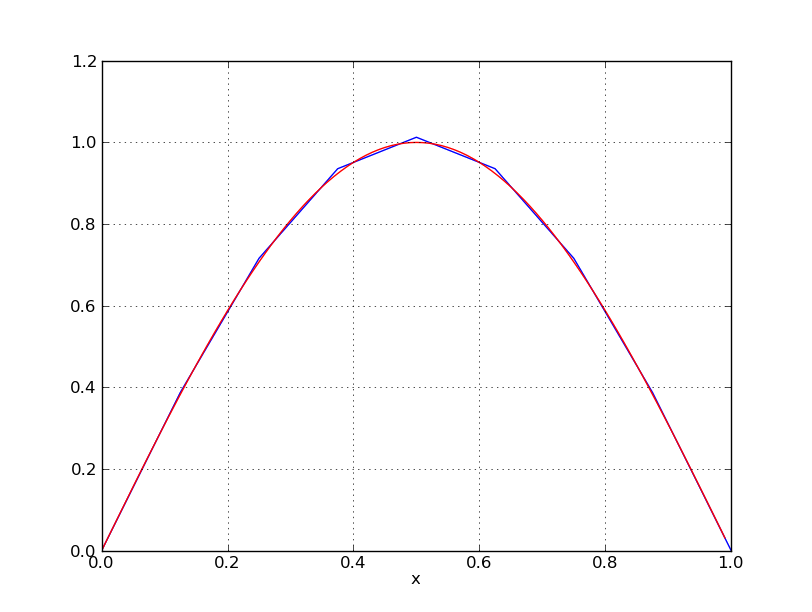
\includegraphics[width=0.55\textwidth]{fig/y_distributed_control_poison_tut_1d_lvl_3_7.png}

\caption{Global solution of $y$ in one dimension. The blue curve is the solution for refinement level 3 and the red one for refinement level 7.}
\label{y_1D}
\end{figure}

\begin{figure}[h!]
	\centering

		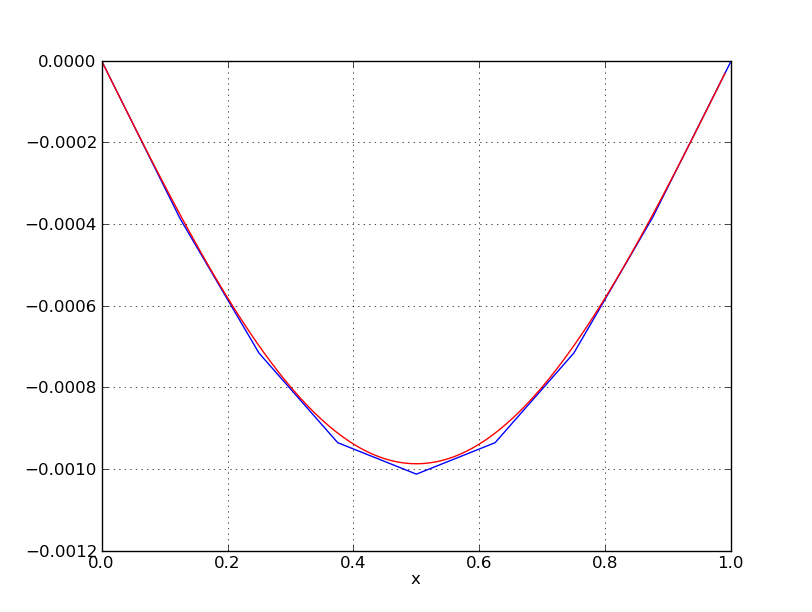
\includegraphics[width=0.55\textwidth]{fig/p_distributed_control_poison_tut_1d_lvl_3_7.png}

\caption{Global solution of $p$ in one dimension. The blue curve is the solution for refinement level 3 and the red one for refinement level 7.}
\label{p_1D}
\end{figure}

\begin{figure}[h!]
	\centering
		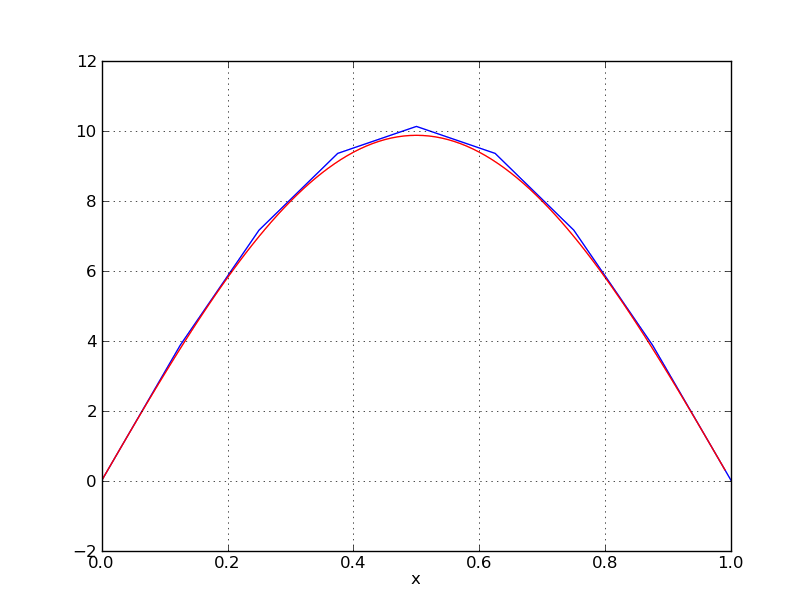
\includegraphics[width=0.55\textwidth]{fig/u_distributed_control_poison_tut_1d_lvl_3_7.png}
\caption{Global solution of $u$ in one dimension. The blue curve is the solution for refinement level 3 and the red one for refinement level 7.}
\label{u_1D}
\end{figure}

\newpage

\subsection{2D Case}\label{sectiontwodimensions}
In this subsection we expand the problem from section \ref{sectiononedimension} to two dimensions and choose now
\begin{eqnarray}
y_{\Omega}(x, y) &=& (1 + 4\lambda \pi^4) \sin (x \pi)  \sin (y \pi), \\
\lambda &=& 0.000001, \\
f(x, y) &=& 0
\end{eqnarray}
and the homogeneous Dirichlet data on the boundary of the unit square $\Omega:=(0,1)\times(0,1)$. The analytical solution is now given by 
\begin{eqnarray}\label{analyticalsolution}
\begin{array}{rcl}
y(x, y) &=& \sin (x\pi) \sin (y\pi), \\
p(x, y) &=& -2 \lambda \pi^2 \sin (x\pi)\sin (y\pi), \\
u(x, y) &=& 2 \pi^2 \sin (x\pi) \sin (y\pi).
\end{array}
\end{eqnarray}
Obviously, $u \in C^2(\Omega) \cap C_0(\overline{\Omega})$ holds since $\sin$ is an analytic function and the product of two analytical functions still is analytical.
The fig. \ref{y_2d} - \ref{u_2d} show the visualized solution for $y$, $p$ and $u$ for refinement level 3 and 7.

\begin{figure}[h!]
	\centering
	\subfigure[Refinement level 3.]{
		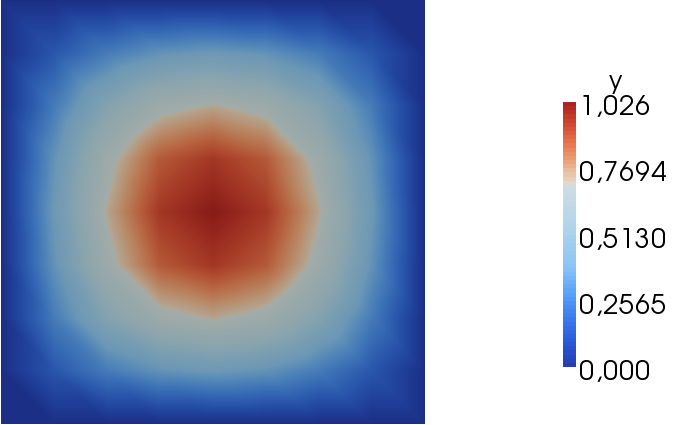
\includegraphics[width=0.45\textwidth]{fig/y_distributed_control_poisson_tut_2d_lvl3_trans.png}
	}
	\subfigure[Refinement level 7.]{
		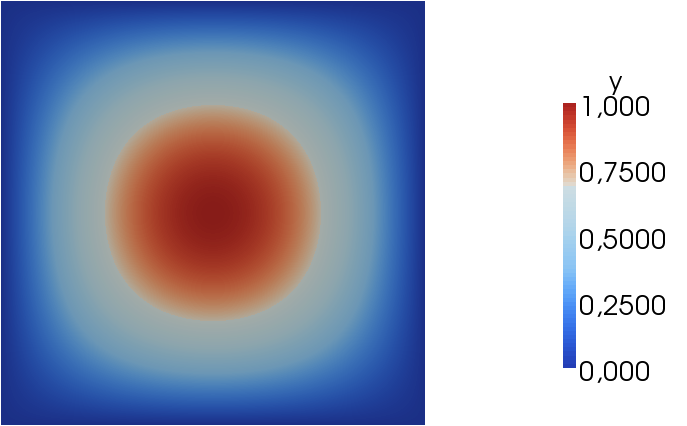
\includegraphics[width=0.45\textwidth]{fig/y_distributed_control_poisson_tut_2d_lvl7_trans.png}
	}
\caption{Global solution of $y$ in two dimensions.}
\label{y_2d}
\end{figure}

\begin{figure}[h!]
	\centering
	\subfigure[Refinement level 3.]{
		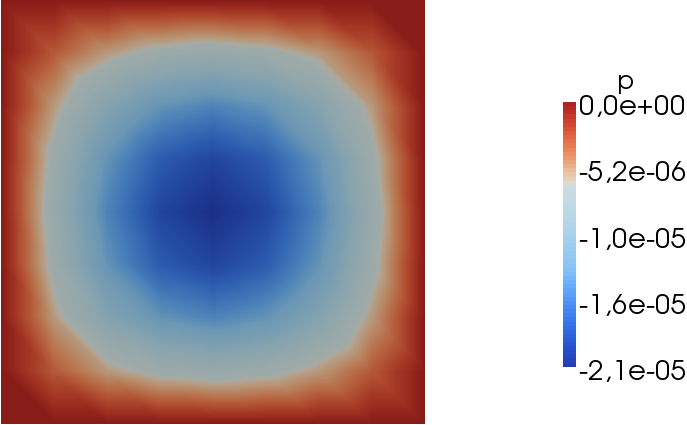
\includegraphics[width=0.45\textwidth]{fig/p_distributed_control_poisson_tut_2d_lvl3_trans.png}
	}
	\subfigure[Refinement level 7.]{
		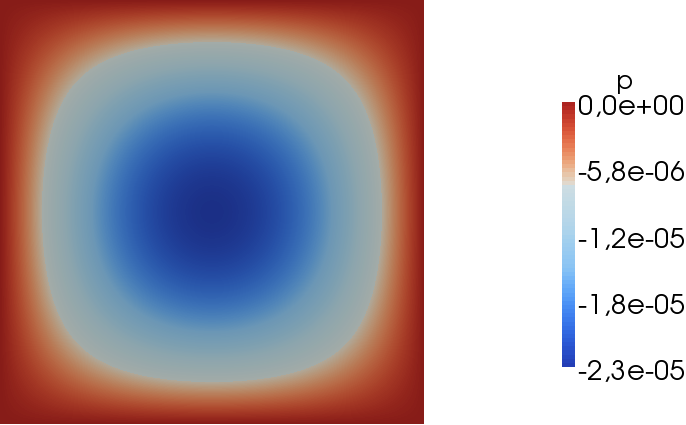
\includegraphics[width=0.45\textwidth]{fig/p_distributed_control_poisson_tut_2d_lvl7_trans.png}
	}
\caption{Global solution of $p$ in two dimensions.}
\label{p_2d}
\end{figure}

\begin{figure}[h!]
	\centering
	\subfigure[Refinement level 3.]{
		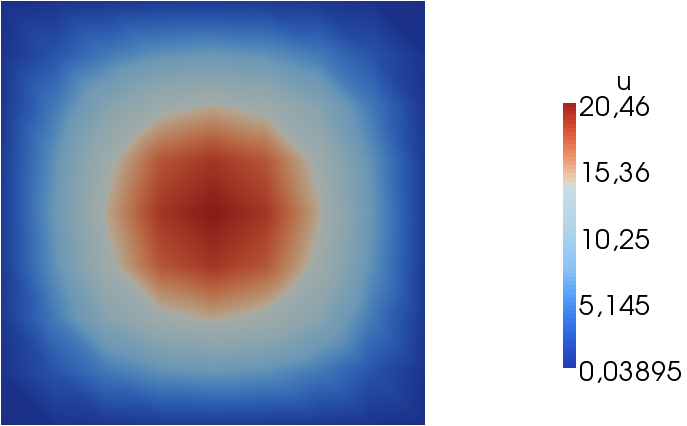
\includegraphics[width=0.45\textwidth]{fig/u_distributed_control_poisson_tut_2d_lvl3_trans.png}
	}
	\subfigure[Refinement level 7.]{
		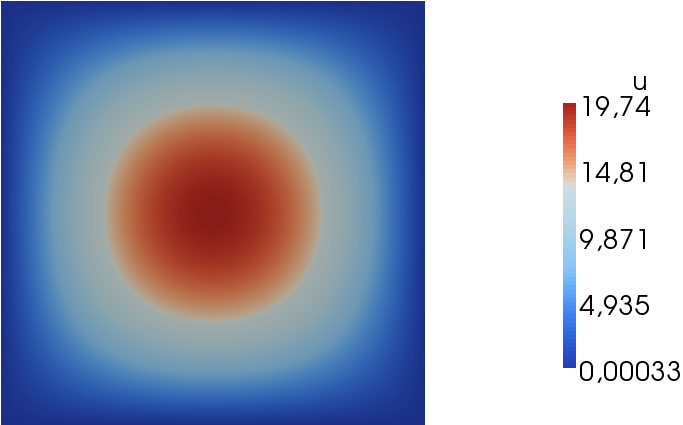
\includegraphics[width=0.45\textwidth]{fig/u_distributed_control_poisson_tut_2d_lvl7_trans.png}
	}
\caption{Global solution of $u$ in two dimensions.}
\label{u_2d}
\end{figure}


\newpage
\section{Quality of the Approximation}
You can find detailed informations about the quality of the approximation by finite element methods in the Poisson tutorial. In this section we just to show the convergence rate of the approximation if you refine the mesh uniformly.
In (\ref{errorplot}) you can see the development of the errors from section \ref{sectiontwodimensions}, if the mesh is uniformly refined. \\


\subsection{Error Plot}\label{errorplot}
In this section the error of example \ref{sectionExample} in the $L^2$-Norm is shown. As one can clearly see in figure \ref{error_plots} the total error is getting smaller, as the refinement level gets higher, which means that the mesh is divided into more cells. One can even see that the error, if drawn in a logarithmic scale behaves kind of linear to the number of cells, which leads to the conclusion that the formula 

\begin{equation}
\mu = \frac{1}{N} \cdot C,
\end{equation}
where $C$ is a constant and N is the number of cells if the refined, approximates the error. Since in two dimensions $N = \frac {1}{\sqrt{h}}$ it holds that
\begin{equation}
\mu = h^2 \cdot C.
\end{equation}

\begin{figure}[h!]
	\centering
	\subfigure[Total $L^2$-error]{
		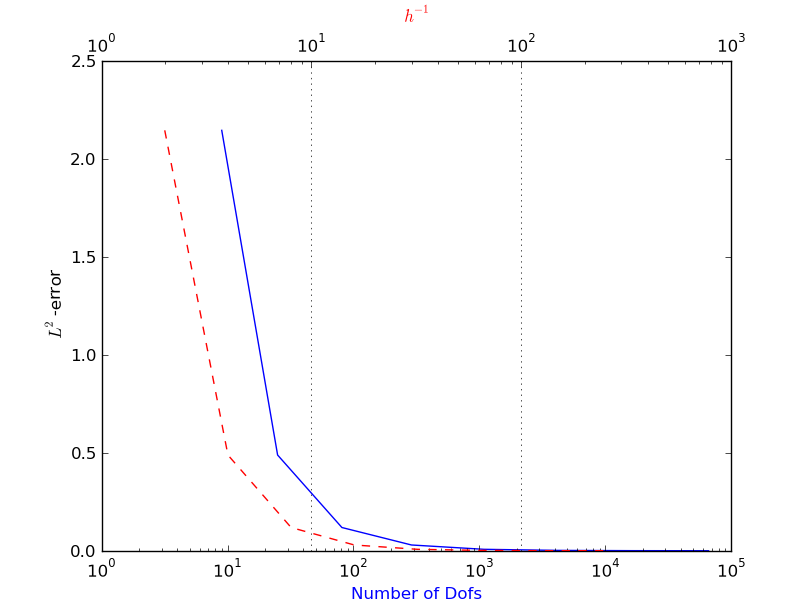
\includegraphics[width=0.45\textwidth]{fig/log_x_error.png}
	}
	\subfigure[Total $L^2$-error on a logarithmic scale]{
		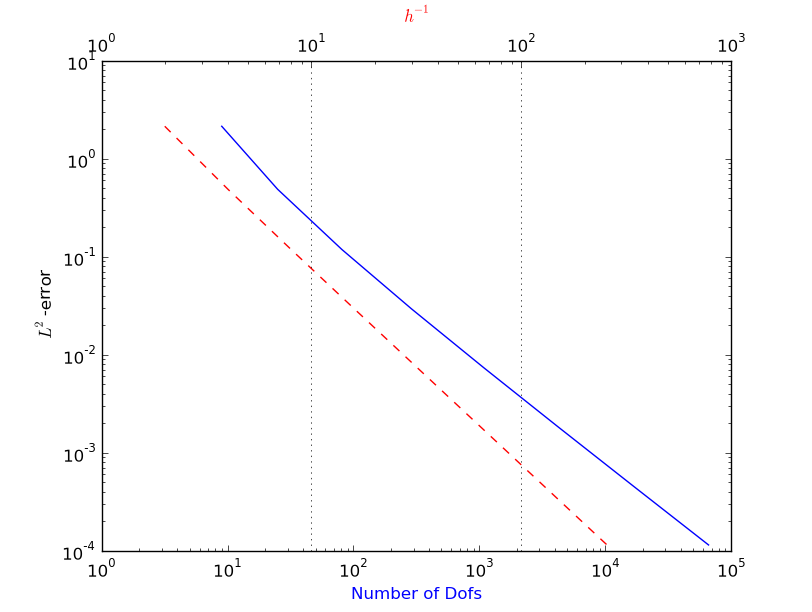
\includegraphics[width=0.45\textwidth]{fig/loglog_error.png}
	}
\caption{Global $L^2$-error in two dimensions.}
\label{error_plots}
\end{figure}

\newpage
\appendix

\bibliography{tutorials_bib}
\bibliographystyle{plain}

\printindex

\end{document}
